\hypertarget{Unit5_8cpp}{
\section{/PIWO/Program/Unit5.cpp File Reference}
\label{Unit5_8cpp}\index{/PIWO/Program/Unit5.cpp@{/PIWO/Program/Unit5.cpp}}
}
{\tt \#include $<$vcl.h$>$}\par
{\tt \#include \char`\"{}Unit5.h\char`\"{}}\par


Include dependency graph for Unit5.cpp:\nopagebreak
\begin{figure}[H]
\begin{center}
\leavevmode
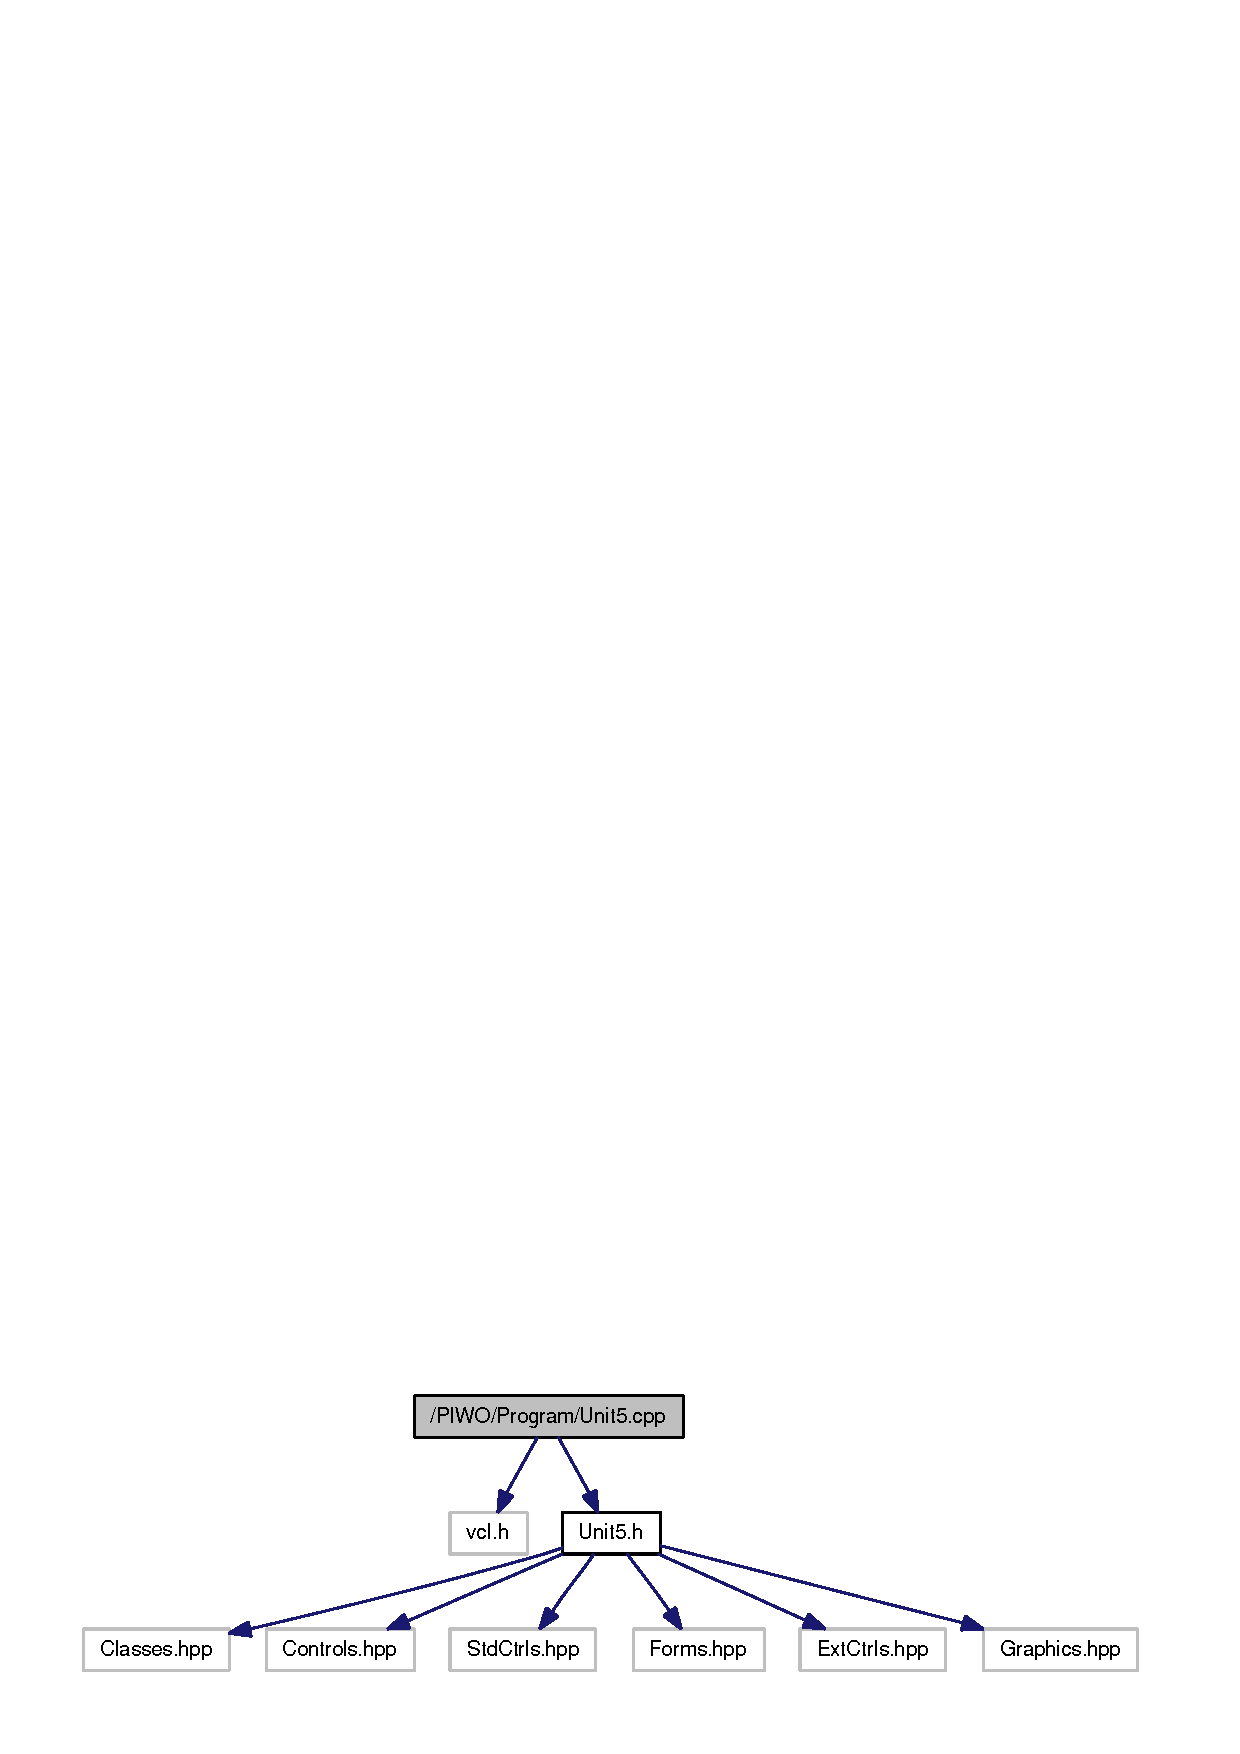
\includegraphics[width=275pt]{Unit5_8cpp__incl}
\end{center}
\end{figure}
\subsection*{Variables}
\begin{CompactItemize}
\item 
\hyperlink{classTForm5}{TForm5} $\ast$ \hyperlink{Unit5_8cpp_caf85d939e9387207488b022c1f9275b}{Form5}
\end{CompactItemize}


\subsection{Variable Documentation}
\hypertarget{Unit5_8cpp_caf85d939e9387207488b022c1f9275b}{
\index{Unit5.cpp@{Unit5.cpp}!Form5@{Form5}}
\index{Form5@{Form5}!Unit5.cpp@{Unit5.cpp}}
\subsubsection[Form5]{\setlength{\rightskip}{0pt plus 5cm}{\bf TForm5}$\ast$ {\bf Form5}}}
\label{Unit5_8cpp_caf85d939e9387207488b022c1f9275b}




Definition at line 11 of file Unit5.cpp.

Referenced by TForm1::Oautorach1Click().